\title{Solutions for Homework 3}
\author{Dr. Jordan Hanson - Whittier College Dept. of Physics and Astronomy}
\date{\today}
\documentclass[10pt]{article}
\usepackage[a4paper, total={18cm, 27cm}]{geometry}
\usepackage{graphicx}
\usepackage{amsmath}
\usepackage{tcolorbox}

\def\rcurs{{\mbox{$\resizebox{.16in}{.08in}{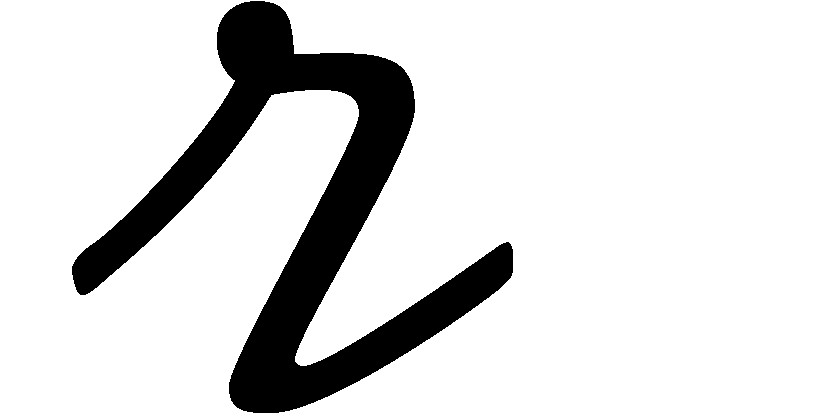
\includegraphics{ScriptR}}$}}}
\def\brcurs{{\mbox{$\resizebox{.16in}{.08in}{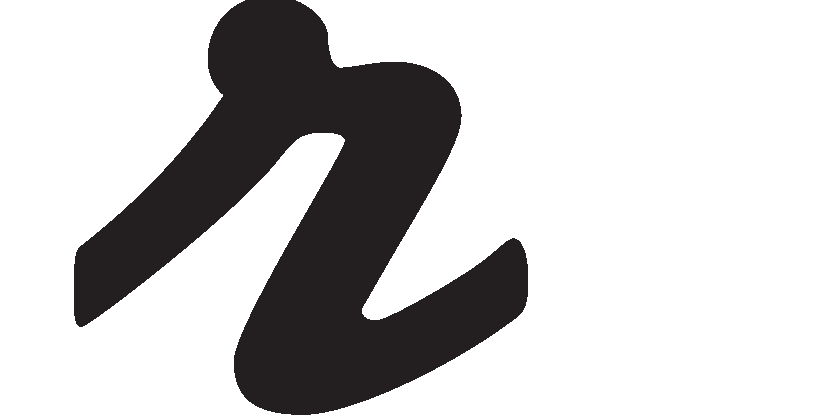
\includegraphics{BoldR}}$}}}
\def\hrcurs{{\mbox{$\hat \rcurs$}}}

\begin{document}
\maketitle

\section{Problem 3.3}

The Laplacian in spherical coordinates, assuming $V(\mathbf{r})$ depends only on $r$, is

\begin{equation}
\frac{1}{r^2}\frac{\partial}{\partial r}\left( r^2 \frac{\partial V}{\partial r}\right) = 0
\end{equation}

\begin{itemize}
\item Multiply both sides by $r$, assuming that $r \neq 0$ (for the Laplacian has a potential singularity there).
\item The quantity $(r^2 dV/dr)$ must be a constant because its derivative is zero.
\item We have
\begin{align}
r^2 \frac{dV}{dr} &= k \\
\frac{dV}{dr} &= \frac{k}{r^2} \\
V(r) &= - \frac{k}{r} + C
\end{align}
Thus the $1/r$ dependence of potential with spherical symmetry is a consequence of Laplace's Equation.  
\end{itemize}

The Laplacian in cylindrical coordinates, assuming $V(\mathbf{r})$ depends only on $s$, is

\begin{equation}
\frac{1}{s}\frac{\partial}{\partial s}\left( s \frac{\partial V}{\partial s}\right) = 0
\end{equation}

Using the same approach as the steps above, we find that $s$ times $dV/ds$ is a constant and that 

\begin{equation}
V(s) = k\ln(s) + C
\end{equation}

Imagine the solution for the potential surrounding a line charge, and notice that it follows this pattern.

\section{Problem 3.5}

\textit{Prove that the field is uniquely determined when the charge density $\rho$ is given and either $V$ or the normal derivative $\partial V/ \partial n$ is specified on each boundary surface.  Do not assume the boundaries are conductors, or that $V$ is constant over any given surface.} \\ \\

This proof follows closely the one on pp. 121-123, with one key difference.  Start by assuming there are two solutions for the field within the volume $\mathcal{V}$ where we find $\rho$.  There is only one $\rho$, but there could be many objects (conductors or otherwise) within the volume, and one global surface containing them all.  The two solutions follow the original reasoning:

\begin{align}
\nabla \cdot \mathbf{E}_1 &= - \frac{\rho}{\epsilon_0} \\
\nabla \cdot \mathbf{E}_2 &= - \frac{\rho}{\epsilon_0} \\
\mathbf{E}_3 &= \mathbf{E}_2 - \mathbf{E}_1 \\
\nabla \cdot \mathbf{E}_3 &= 0 \\
\oint \mathbf{E}_3 \cdot d\mathbf{a} &= 0 ~~ (all ~~ surfaces) \\
\mathbf{E}_3 &= -\nabla V_3 \\
\nabla \cdot (V_3 \mathbf{E}_3) &= V_3 (\nabla \cdot \mathbf{E}_3) + \mathbf{E}_3 (\nabla V_3) = 0 - \mathbf{E}_3 \cdot \mathbf{E}_3 = - E_3^2
\end{align}

Integrate the final line with respect to volume, over $\mathcal{V}$:

\begin{equation}
\int_\mathcal{V} \nabla \cdot (V_3 \mathbf{E}_3) d\tau = -\int E_3^2 d\tau
\end{equation}

Use the divergence theorem on the left-hand side:

\begin{equation}
\oint V_3 \mathbf{E}_3 \cdot d\mathbf{a} = -\int E_3^2 d\tau
\end{equation}

The integrand on the left hand is zero if:

\begin{itemize}
\item The potentials $V_1$ and $V_2$ are specified on each surface.  Then, $V_3$ over each and every surface, and the integrand is zero.
\item The normal derivatives $\partial V_1 / \partial n$ and $\partial V_2 / \partial n$ are specified.  Then, $\partial V_3 / \partial n = -E_{3,\perp} = 0$, and the integrand is zero.
\end{itemize}

Thus, either way, the integrand is zero and 

\begin{equation}
\int E_3^2 d\tau = 0
\end{equation}

That means that $E_3 = 0$, and $\mathbf{E}_2 = \mathbf{E}_1$.  The field is unique.

\section{Problem 3.6}

\textit{A more elegant proof of the second uniqueness theorem uses Green's identity (Problem 1.16c), with $T = U = V$.  Supply the details.} \\ \\

And ... go!

\begin{align}
\int_\mathcal{V} (V_3 \nabla^2 V_3 + \nabla V_3 \cdot \nabla V_3) d\tau &= \oint (V_3 \nabla V_3) \cdot d\mathbf{a} \\
\int_\mathcal{V} (0 + \nabla V_3 \cdot \nabla V_3) d\tau &= - \oint (V_3 \mathbf{E}_3) \cdot d\mathbf{a} \\
- \int_\mathcal{V} E_3^2 d\tau &= - \oint (V_3 \mathbf{E}_3) \cdot d\mathbf{a} \\
\int_\mathcal{V} E_3^2 d\tau &= \oint (V_3 \mathbf{E}_3) \cdot d\mathbf{a}
\end{align}
Using the same logic as the prior exercises completes the proof.

\section{Problem 3.13}

\textit{Find the potential in the infinite slot of Ex. 3.3 if the boundary at $x=0$ consists of two metal strips: one, from $y=0$ to $y=a/2$, is held at a positive constant potential $V_0$, and the other, from $y=a/2$ to $y=a$, is held at a negative constant potential $-V_0$.} \\ \\

Using Ex. 3.3, one can arrive at

\begin{align}
V(x,y) &= \sum_{n = 1}^{\infty} C_n e^{-n \pi x / a} \sin(n \pi y / a) \\
C_n &= \frac{2}{a}\int_0^a V_0(y) \sin(n \pi y / a) dy 
\end{align}

The Fourier coefficient is found by applying the boundary condition:

\begin{equation}
C_n = \frac{2V_0}{a} \left( \int_0^{a/2} \sin(n\pi y/a) dy - \int_{a/2}^{a} \sin(n\pi y/a) dy\right) = \frac{2 V_0}{n\pi}(1+(-1)^n - 2\cos(n\pi/2))
\end{equation}

How do we generalize the result into a sum of solutions?  Notice that the coefficient is zero if (a) $n$ is odd, or (b) $n$ is a multiple of 4.  Otherwise, it turns into $4$.  Thus:

\begin{equation}
C_n = \frac{8V_0}{n\pi}, ~~ n = (4j+2), ~ j = 0,1,2, ...
\end{equation}

The solutions can be gathered into the series above like so:

\begin{equation}
V(x,y) = \frac{8V_0}{\pi}\sum_{j=0}^{\infty} \frac{e^{-(4j+2)\pi x / a} \sin((4j+2) \pi y/a)}{4j+2}
\end{equation}

\end{document}
